
%---- Created by: Sinchiguano Cesar. El Carmen - June 2022 --
\documentclass[xcolor=dvipsnames,envcountsect]{beamer}
%Default package loading
\usepackage{import}
\import{sourceFile/}{source.tex}
\usepackage{graphicx}
\usepackage{caption}
\usepackage{subcaption}

%--------- START DOCUMENT ------------------
\begin{document}
\begin{frame}{\titlepage}\end{frame}
\begin{frame}{\frametitle{Contenido}\tableofcontents}\end{frame}


\section{Perfil del docente}
\begin{frame}
	\frametitle{Perfil del docente}
		\justifying
		
\begin{figure}
     \centering
     \begin{subfigure}[b]{0.3\textwidth}
         \centering
         
\includegraphics[width=\textwidth]{Figures/epn.jpg}
         %\caption{$y=x$}
         %\label{fig:y equals x}
     \end{subfigure}
     \hfill
     \begin{subfigure}[b]{0.3\textwidth}
         \centering
         
\includegraphics[width=\textwidth]{Figures/cvut.jpg}
         %\caption{$y=3sinx$}
         %\label{fig:three sin x}
     \end{subfigure}
     \vfill
     \begin{subfigure}[b]{0.2\textwidth}
         \centering
         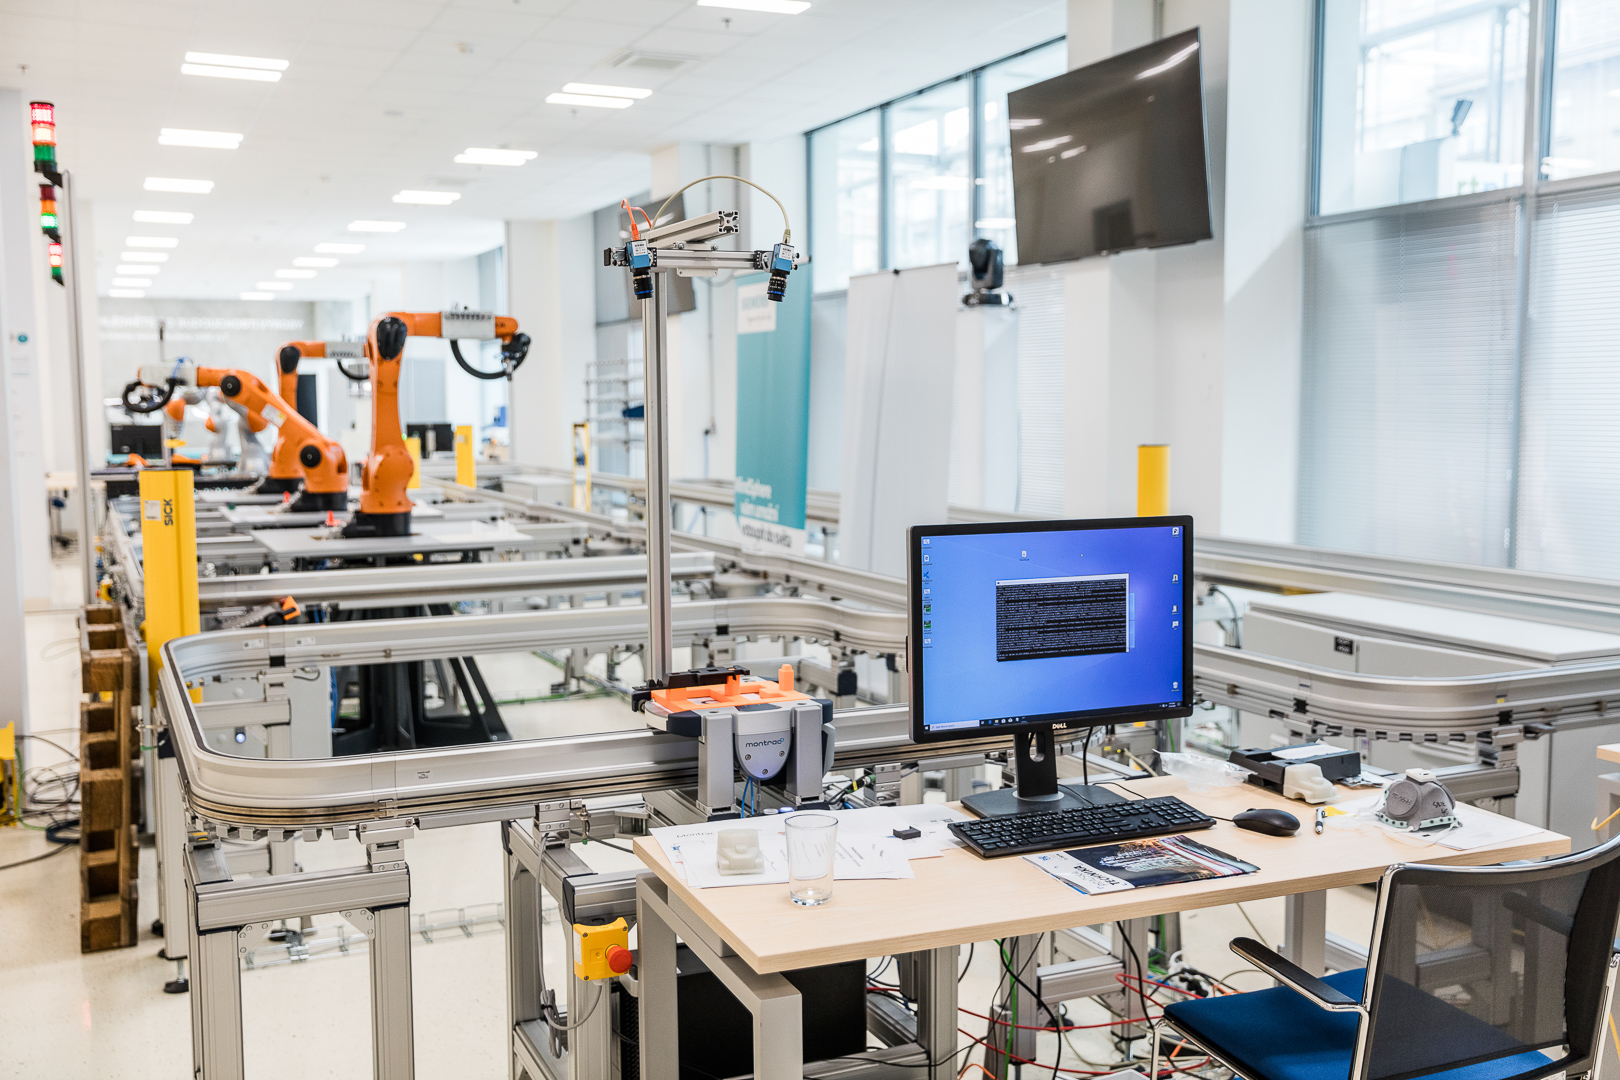
\includegraphics[width=\textwidth]{Figures/ciirc.jpg}
         %\caption{$y=5/x$}
         %\label{fig:five over x}
     \end{subfigure}
        %\caption{Three simple graphs}
        %\label{fig:three graphs}
\end{figure}
\end{frame}



%---------
\section{Consideraciones generales}
\begin{frame}[allowframebreaks]
	\frametitle{Consideraciones generales}
		\justifying

		
		
		
		
		
		
		\begin{enumerate}
		\item Clases de 4-Agosto-2022 hasta 26-Agosto-2022
			  \begin{enumerate}
			  \item[A)] Primer parcial (9 días)
				   \begin{enumerate}
				   \item  4-Agosto hasta 13-Agosto	
				   \item Proyecto      			$30\%$
				   \item Evaluaciones continua  $20\%$
				   \item Exposiciones 			$20\%$
				   \item Examen final 			$30\%$ 	
				   \end{enumerate}
			   \item[B)] Segundo parcial (9 días)
			 	    \begin{enumerate}
			 		\item 15-Agosto hasta 24-Agosto
				    \item Proyecto      			$30\%$
				    \item Evaluaciones continua  $20\%$
				    \item Exposiciones 			$20\%$
				    \item Examen final 			$30\%$ 	
				     \end{enumerate}
			   \item[C)] Recuperación (2 días)
			 	    \begin{enumerate}
			 		\item 25-Agosto, 26-Agosto
				    \item Examen 			$100\%$ 	
				     \end{enumerate}
				\end{enumerate}
		\item Proyecto primer parcial
				\begin{enumerate}
				
				\item Tema
					\begin{enumerate}
					\item Informe (3 a 5 hojas)
					\item Exposición teórica y práctica 
					\end{enumerate}
				\item Presentación (12-Agosto-2022) 
				\item Práctica (13-Agosto-2022)
				\end{enumerate}
		\item Proyecto segundo parcial
				\begin{enumerate}
				
				\item Tema
					\begin{enumerate}
					\item Informe (3 a 5 hojas)
					\item Exposición teórica y práctica 
					\end{enumerate}
				\item Presentación (23-Agosto-2022) 
				\item Práctica (24-Agosto-2022)
				\end{enumerate}
		\end{enumerate}

			
		
		
\end{frame}








%-------------------------------------
\section{Sílabo}
\begin{frame}
	\frametitle{Sílabo}
		\justifying
		\begin{enumerate}
		\item Fundamentos eléctricos.
			\begin{enumerate}
			\item Instalaciones eléctricas
			\item Tipos de instalaciones eléctricas
			\item Corriente AC y CC
			\item Red de transporte y distribución eléctrica
			\end{enumerate}
		\item Diseño de instalaciones
			\begin{enumerate}
			\item Definiciones
			\item Marco normativo y referencias
			\item Instalación eléctrica de la vivienda BT
			\item Instalación de enlace
			\item Instalación interior de la vivienda
			\end{enumerate}
		\item Domótica aplicada.
			\begin{enumerate}
			\item Definición
			\item Instalación domótica
			\item Estructura de un sistema domótico
			\item Salidas y entradas del sistema domótico
			\item Sistemas domóticos comerciales
			\item Controla tu hogar con arduino
			\begin{enumerate}
				\item Ambiente arduino
				\item Programación en C
				\item Programación en arduino 
			\end{enumerate}		
			\end{enumerate}
		\item Simulaciones eléctricas.
			\begin{enumerate}
			\item TINKERCAD
			\item LED parpadeante
			\item LCD mensaje
			\end{enumerate}
		\end{enumerate}
\end{frame}



%---------
\section{Fundamentos eléctricos}
\begin{frame}
	\frametitle{Fundamentos eléctricos}
		\justifying
		\begin{enumerate}
			\item Instalaciones eléctricas
			\item Tipos de instalaciones eléctricas
			\item Corriente AC y CC
			\item Red de transporte y distribución eléctrica
			\begin{enumerate}
			\item El viaje de la electricidad
			\end{enumerate}
		\end{enumerate}
\end{frame}


%-------------------------------
\section{Diseño de instalaciones}
\begin{frame}
	\frametitle{Diseño de instalaciones}
		\justifying
		\begin{enumerate}
			\item Definición
			\item Marco normativo y referencia
			\item Instalación eléctrica de la vivienda
			\item Instalación de enlace
			\item Instalación interior de la vivienda
		\end{enumerate}
\end{frame}



%---------- 
\section{Domótica aplicada}

\begin{frame}
		\frametitle{Domótica aplicada}
		\begin{enumerate}
			\item Definición
			\item Instalación domótica
			\item Estructura de un sistema domótico
			\item Salidas y entradas del sistema domótico
			\item Sistemas domóticos comerciales
			\item Controla tu hogar con arduino
			\begin{enumerate}
				\item Ambiente arduino
				\item Programación en C
				\item Programación en arduino 
			\end{enumerate}			
		\end{enumerate}				
\end{frame}


%----------- 
\section{Simulaciones eléctricas}
\begin{frame}{Simulaciones eléctricas}
		\begin{enumerate}
			\item TINKERCAD
			\item LED parpadeante
			\item LCD mensaje
		\end{enumerate}		
\end{frame}





%--------- THANK YOU Text --------------------------
	\begin{frame}
		\centering
		\begin{block}
			\scshape
				\begin{center}
					\Huge\emph{Gracias!}
				\end{center}
		\end{block}
	\end{frame}
%----------------------------------------------------
\end{document}
